\documentclass[conference]{IEEEtran}
\IEEEoverridecommandlockouts
% Default IEEE packages
\usepackage{cite}
\usepackage{amsmath,amssymb,amsfonts}
\usepackage{algorithmic}
\usepackage{graphicx}
\usepackage{textcomp}
\usepackage{xcolor}
\def\BibTeX{{\rm B\kern-.05em{\sc i\kern-.025em b}\kern-.08em
    T\kern-.1667em\lower.7ex\hbox{E}\kern-.125emX}}
    
% Additional packages
\usepackage{multirow}
\usepackage{tikz}

\newcommand{\xs}{-1}
\newcommand{\ys}{0.5}

% Tikz commands
\newcommand{\cube}[6]{  % 2 x-y, 3 dimensions, 1 color
        \begin{scope}[
        	shift={(#1, #2)},
			yslant=\ys ,xslant=\xs
            ]
            \filldraw[fill=#6] (0,0) rectangle (#3, #4);
            \draw[black] (0,0) rectangle (#3,#4);%marking borders
        \end{scope}
        \begin{scope}[
        	shift={(#1, #2)},
            yslant=\ys ,xslant=0
            ]
            \filldraw[fill=#6] (0,0) rectangle (#3, -#5);
            \draw[black] (0,0) rectangle (#3,-#5);%marking borders
        \end{scope}
        \begin{scope}[
        	shift={(#1, #2)},
            yslant=-\ys ,xslant=0
            ]
            \filldraw[fill=#6] (0,0) rectangle (-#4, -#5);
            \draw[black] (0,0) rectangle (-#4,-#5);%marking borders
        \end{scope}
}

\newcommand{\gridcube}[6]{  % 2 x-y, 3 dimensions, 1 color
        \begin{scope}[
        	shift={(#1, #2)},
            every node/.append style={
            yslant=0.5,xslant=-1},yslant=0.5,xslant=-1
            ]
            \filldraw[fill=#6] (0,0) rectangle (#3, #4);
            \draw[step=1, black!50] (0,0) grid (#3,#4); %defining grids
            \draw[black,very thick] (0,0) rectangle (#3,#4);%marking borders
        \end{scope}
        \begin{scope}[
        	shift={(#1, #2)},
            every node/.append style={
            yslant=0,xslant=0},yslant=0.5,xslant=0
            ]
            \filldraw[fill=#6] (0,0) rectangle (#3, -#5);
            \draw[step=1, black!50] (0,0) grid (#3,-#5); %defining grids
            \draw[black,very thick] (0,0) rectangle (#3,-#5);%marking borders
        \end{scope}
        \begin{scope}[
        	shift={(#1, #2)},
            every node/.append style={
            yslant=0,xslant=0},yslant=-0.5,xslant=0
            ]
            \filldraw[fill=#6] (0,0) rectangle (-#4, -#5);
            \draw[step=1, black!50] (0,0) grid (-#4,-#5); %defining grids
            \draw[black,very thick] (0,0) rectangle (-#4,-#5);%marking borders
        \end{scope}
}

\newcommand{\tikzcircle}[2][red,fill=red]{\tikz[baseline=-0.5ex]\draw[#1,radius=#2] (0,0) circle ;}%

    
\begin{document}

\title{Curvy DeepPicar
\thanks{Accompanying GitHub Repo: https://github.com/p678m854/EECS-753-Project}
}

\author{\IEEEauthorblockN{Patrick McNamee}
\IEEEauthorblockA{\textit{Department of Electrical Engineering and Computer Science} \\
\textit{University of Kansas}\\
Lawrence, KS \\
p678m854@ku.edu}}

\maketitle

\begin{abstract}

Convolutional Neural Networks (CNN) are a common implementation for vision based driving on autonomous vehicles. One common technical issue for these CNN vision based systems is that the neural network outputs tend to be very noise with no guarantees of output smoothness as the vehicle traverses the environment. Previous work has shown that using the network outputs as B\`ezier curves for an outer loop navigation controller with an inner pursuit curve controller leads to smooth performances and outperform other network architectures. This work follows a natural extension implements a CNN with B\`ezier curve outputs as part of the controller module rather navigational module on a physical platform for vision navigation and evaluates the results against a standard CNN as a direct controller.

\end{abstract}

\begin{IEEEkeywords}
machine learning, autonomous vehicles, embdedded platforms, guidance navigation and control
\end{IEEEkeywords}

\section{Introduction}

Modern car manufacturers are developing autonomous automobiles for future use in both civilian and military applications. There are various complex environmental aspects that are required for consideration in order for autonomous agents to succeed in driving tasks such as sensors for object detection and localization, path planning, and state prediction for object avoidance \cite{kato2018}. These aspects traditionally rely on computationally complex and resource intensive algorithms that may be too slow to implement on a real-time system. An alternative is to use neural networks which are universal approximators \cite{wang2021interval} to approximate the algorithms for a loss of functional accuracy but an increase in computational throughput. As such, neural networks have been frequently used for autonomous vehicle.

Usage of neural networks in autonomous ground vehicles has been around for decades with ALVINN being one of the first examples of vision-based navigation \cite{pomerieau-1989}. ALVINN used a 32 by 32 video input along with a 8 by 32 range finder input feed into a hidden layer of 29 units before the output layer of 46 units. The wheel steering angle was chosen based on the values of the 46 output units and ALVINN was quite successful at its various driving tasks. Modern implementations of autonomous cars, like the one developed by NVIDIA, are empowered by modern computational performance have since moved from the relatively simple network architecture used in ALVINN and currently use CNN which includes convolutional layers as well as significantly larger layers size \cite{bojarski2016end}. While these larger neural networks have allowed for more complex behavior of the autonomous agent, there are still issues that result from the nature of neural networks. Often the outputs of neural networks are rough in the sense  small manipulations on the input layer can produce drastically different outputs and there are no guarantees of output behavior in unexplored environments. Still, CNNs are potential methods to work towards fully autonomous driving and there are several implementation techniques to include them.

\subsection{Background}

There are various ways for CNNs to be implemented for autonomous vision-based automobile navigation as reference in Fig. \ref{fig:vb-steering}. The most direct method is to have the CNN take images and translate them into direct control inputs such as the steering angle or throttle as in \cite{bechtel2018}. While direct, this implementation is limited in that the controller is limited by the input rate of the camera systems as well as the network throughput implementation. It is also susceptible to network output roughness which can lead to high control jerk and unnecessarily fatigued physical components. This implementation of a direct controller is referred to in the rest of this work as image-to-point for translating a camera image into a point in the control dimensional space.

Two alternative implementations that are indirect schemes are navigational implementations as implemented in DeepRacing \cite{trent2020iros}. Rather than directly control the car, the CNN outputs desired positions to navigate with a lower level control scheme closing the loop. There are two different ways to represent navigational points using discrete and continuous methods. A discrete method is simply to transform the input into a collection of ordered waypoints for navigation. However, a CNN with rough outputs will still produce noisy outputs that may cause unwanted behavior. Additionally as the number of waypoints changes, the network architecture needs to be adjusted.

Rather than represent the waypoints or as discrete points, the waypoints can be represented as a continuous polynomial curves. B\`ezier curves $\mathbf{B}$ are useful representation as any polynomial of degree $d$ can be implemented with $d+1$ points $\mathbf{P}_k$ in $k$ dimensional space as poles by \eqref{eq:bezier-curve} using a parameter $t$.

\begin{equation}
\label{eq:bezier-curve}
\mathbf{B}(t) = \sum_{k=0}^{d} \genfrac(){0pt}{0}{d}{k} (1-t)^{d-k}t^k \mathbf{P}_k \quad t\in [0, 1]
\end{equation}

This representation is advantageous as it can represent the same time window as the discrete waypoint representation but has an infinite number of points so the number of waypoints generated is not upper bounded. Additionally the waypoints are guaranteed to be smooth since they are on a polynomial curve and experimentally DeepRacing showed that this B\`ezier representation was the best performing network for CNN in the simulated racing domain \cite{trent2020iros} but not any physical platform.

\begin{figure}[hbtp]
	\centerline{
	\begin{tikzpicture}
		% labeling
		\node at (-1.5,4) {a)};
		\node at (-1.5,2) {b)};
		\node at (-1.5,0) {c)};
		
		% Plot the basic images
		\foreach \y in {0,2,4}{
			\node at (0,\y) {\includegraphics[width=1.5cm,height=1cm]{..//figures/presentation/out-video-1-moment.jpg}};  % Image from camera
			\draw[blue, ultra thick, -latex] (0.8,\y) -- (1.45,\y);
			\filldraw[black, fill=black!60] (1.5,\y-0.25) rectangle node[white] {CNN} (2.5,\y+0.25);  % Neural Network
			\draw[red, ultra thick, -latex] (2.6,\y) -- (3.1,\y);
		}
		% Image-to-Point
		\draw (3.2,4) node[anchor=west] {$\theta_{\text{steering}} = 30^\circ$};
		% Image-to-Waypoints
		\draw[black, latex-latex] (3.2,1.5) -- (3.2, 2.5) node[anchor=south]{$y$};
		\draw[black, -latex] (3.2,2) -- (5,2) node[anchor=west]{$x$};
		\foreach \dx in {0.1,0.3,...,1.5}
			{\filldraw[red, fill=red] ( 3.2 + \dx , {2 - 0.15*pow(\dx, 2)} ) circle (1.5pt);}
		% Image-to-Curve
		\draw[black, latex-latex] (3.2,-0.5) -- (3.2, 0.5) node[anchor=south]{$\theta$};
		\draw[black, -latex] (3.2,0) -- (5,0) node[anchor=west]{$t$};
		\draw[red] (3.2,0) .. controls (3.75,0.5) and (4.25,-0.5) .. (4.9,-0.2);
		\draw[red] (3.2,0) circle (1.5pt);
		\draw[red] (3.75,0.5) circle (1.5pt);
		\draw[red] (4.25,-0.5) circle (1.5pt);
		\draw[red] (4.9,-0.2) circle (1.5pt);
		
	\end{tikzpicture}
	}
	\caption{Various Vision-Based Autonomous Steering Implementations. From top to bottom; a) image to direct control command, b) image to localized waypoints (\tikzcircle{2pt}), and c) image to curve using poles ({\color{red} $\circ$}).}
	\label{fig:vb-steering}
\end{figure}

While most work is focused on personal or racing automobiles, there have been implementations of vision-based navigation on small, radio-controlled cars. These vehicles are significantly cost-effective as research platforms and test embedded systems. Previous work at the University of Kansas has demonstrated implementing the NIVIDIA DAVE-2 neural network architecture on a Raspberry Pi for a CNN image-to-point vision navOutline of track used.
Mention how code was changed.
Give some results. igation system \cite{bechtel2018}. From a cost standpoint, the DeepPicar platform is ideal for testing a real implementation of a CNN with B\`ezier curve output although due to hardware and sensor limitations, an image-to-curve controller will need to used to compare the B\`ezier implementation of a controller against a standard image-to-point CNN controller rather than having the B\`ezier CNN be the navigational controller as in \cite{trent2020iros}.

\subsection{Motivations}

Previous work has shown the use of CNNs outputting B\`ezier curves for navigation problems in simulated racing outperforms other techniques such as a CNN outputting navigation waypoints or direct control networks \cite{trent2020iros}. However the simulation relies on position estimates which may not be feasible onboard small platforms or in environments with no direct position estimates and the B\`ezier curve outputs have, to the knowledge of the author, not been tested on a physical platform currently. Hence this work seeks to implement the a CNN outputting B\`ezier curves in a direct control scheme for navigating a track on the DeepPicar.

\section{Novel Contributions}

This work will implement a CNN outputting B\`ezier control curves for an embedded autonomous automobile platform for course navigation which has not been tested before on a physical platform or as a direct control command. This new implementation will be tested against a standard CNN with direct control output as used in previous work \cite{bechtel2018} on the same physical platform.

\section{Convolutional Neural Networks}

\begin{figure*}[bt]
	\centerline{
		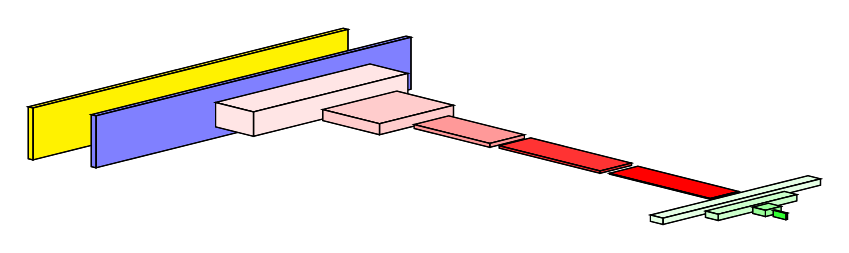
\begin{tikzpicture}[yscale=0.01, xscale=0.02]
		\cube{0}{0}{200}{3}{66}{yellow}
		\cube{40}{-10}{200}{3}{66}{blue!50}
		\cube{140}{-5}{98}{24}{31}{red!10}
		\cube{220}{-20}{47}{36}{14}{red!20}
		\cube{290}{-45}{22}{48}{5}{red!40}
		\cube{360}{-80}{20}{64}{3}{red!80}
		\cube{430}{-115}{18}{64}{1}{red}
		\cube{400}{-140}{100}{8}{8}{green!10}
		\cube{435}{-135}{50}{8}{8}{green!20}
		\cube{465}{-130}{10}{8}{8}{green!40}
		\cube{478}{-134}{1}{8}{8}{green!80}
		\end{tikzpicture}
	}
	\caption{Visualization of DAVE-2 Neural Network \cite{bojarski2016end}. Yellow is an input image, blue is the regularization layer, red is a convolution layer, and green is a dense layer. Dense layers are exaggerated for viewing and flattening omitted.}
	\label{fig:dave-2}
\end{figure*}

The CNNs are based off of the DAVE-2 CNN architecture from NIVIDIA \cite{bojarski2016end} and is shown in Fig. \ref{fig:dave-2}. Previous work has been implemented on a Raspberry Pi for the DeepPicar \cite{bechtel2018} and this work will use the same implementation as \cite{bechtel2018} to form a direct comparison with previous implementations. The input to the CNNs is a Playstation Eye Camera which generates $320\times 240$ RGB image frames which are resized to $200\times 66$ to match the DAVE-2 inputs. Inside the CNNs, the image is normalized across the image width, height, and channels before passing though multiple convolution layers. Layers 2, 3, and 4 use $5\times 5$ kernels with a width and height stride of $(2,2)$ while layers 5 and 6 use $3\times 3$ kernels with a width and height stride of $(1,1)$. After layer 6, the network is flattened to dense layers whose layer width is reduced until a single output unit. The activation functions used for layers 2 through 10 are rectilinear linear units (ReLU) while the last layer uses a hyperbolic tangent function. These activation functions are consistent with implementations in previous work \cite{bechtel2018,bojarski2016end} but the use of ReLU for the hidden layers are consistent with proofs that neural networks are universal approximators \cite{HORNIK1989359} and the hyperbolic tangent allows for outputs to be bounded to match the automobiles steering wheel angle limits $ [\theta_{\min},\ \theta_{\max}] $ by a linear transformation.

\subsection{Training Datasets}


There are two publicly datasets available, and investigated, to train radio-control autonomous cars for tracks. The first dataset is a popular, non-academic, but relatively small and non-timestamped dataset consisting of only 219 example images but has a continuous steering angle ranging \cite{tian2019} while the other dataset consists of 11,000 timestamped example images but only has a collection of discrete wheel angles in the set $\lbrace -30^\circ,\ 0^\circ,\ 30^\circ \rbrace$ degrees but uses the same physical platform as this work \cite{bechtel2018}. As the B\`ezier curves deal with continuous outputs, it would be more advantageous from a training perspective to attempt to use Data Augmentation to train the various CNN models on the first dataset and then evaluate the CNN models on the larger second dataset to see if any trained model can be transferred to the matching physical platform. For the training on \cite{tian2019}, all images were loaded into memory and an application of a horizontal image flight was applied to augment the dataset. The target steering wheel angles were scaled so that the models was only attempting to output in the range $[-1,\ 1]$ where $-1$ and $1$ indicate a steering wheel angle of $-30^\circ$ degrees and $30^\circ$ i.e. $30^\circ$ left and right respectively. For train the CNN whose architecture is in Table \ref{tab:i2c-arch}, a 80-20 test-validation set split was used with a mean squared error (MSE) loss function and the model was trained for 100 epochs using the ADAM optimizer with parameters in Table \ref{tab:training-parameters}.

\begin{figure}[tbhp]
	\centerline{\includegraphics[width=1.5in]{"../../data/external/DeepPicar-data/video01_000_085.png"}\hspace*{0.1in}\includegraphics[width=1.5in]{../figures/presentation/out-video-1-moment.jpg}}
	\caption{Examples from the datasets where left is from \cite{tian2019} and right is from \cite{bechtel2018}.}
\end{figure}

\begin{table}[btp]
        \centering
            \caption{Image-to-Point CNN Model using Domain Augmentation (Acc: 38.71\%)}
            \begin{tabular}{|c|r|c|c|c|}
            \multicolumn{2}{c}{} & \multicolumn{3}{c}{\bfseries Model Predicted}\\\cline{3-5}
            \multicolumn{1}{c}{} & & \textbf{\textit{Left}} & \textbf{\textit{Center}} & \textbf{\textit{Right}}\\\hline
             \parbox[t]{2mm}{\multirow{3}{*}{\rotatebox[origin=c]{90}{\bfseries Record}}} & \textbf{\textit{Left}} & 141 & 1,147 & 28 \\\cline{3-5}
            & \textbf{\textit{Center}} & 820 & 3,334 & 306 \\\cline{3-5}
            & \textbf{\textit{Right}} & 850 & 3,591 & 783 \\\cline{3-5}\hline
            \end{tabular}
        \label{tab:i2p-da-acc}
    \end{table}

To analyze the performance of the model in the new domain of \cite{bechtel2018} which has a discrete controller, the CNN model was used to predict the continuous wheel angle for all 1,000 frames of each of the 11 videos and the output was rounded to the closes steering angle in $\lbrace -30^\circ,\ 0^\circ,\ 30^\circ \rbrace$. A cross-correlation matrix of the model outputs versus the record steering wheel angles are displayed in Table \ref{tab:i2p-da-acc}. The accuracy was not deemed high enough to use the model in the domain of \cite{bechtel2018} which has the same physical platform of this work so data augmentation cannot be used in this work. However, the \cite{bechtel2018} dataset outputs still need to be  modified to appear to be continuous. To achieve this effect, the CNN models will train on a central moving average filter of the steering wheel angles with a filter window of 5 data points which are nominally spaced at 50 milliseconds.

\subsection{Image-to-Point CNN}

The image-to-point CNN is a recreation of the models trained in previous work \cite{bechtel2018,bojarski2016end} with the various layers types, dimensions, and total parameters listed in Table \ref{tab:i2p-arch}. There is a discrepancy between the original DeepPicar previous work \cite{bechtel2018} and \cite{bojarski2016end} where the first normalization layer is excluded from the CNN. Since the original DeepPicar was using the DAVE-2 CNN as the reference model, this work will also follow the DAVE-2 model and include the layer normalization. For training, the CNN will use the mean squared error (MSE) loss function with the recorded wheel angles being proportionally scaled to the range $[1, -1]$. Afterwards, the model will be implemented onto the DeepPicar as an image-to-point navigation controller operating at 20 Hz.

\begin{table}[tbp]
	\centering
	\caption{Image-to-Point Convolutional Neural Network Architecture}
	\begin{tabular}{|r|c|c|r|}
	\multicolumn{1}{c}{\bfseries Layer} & \multicolumn{1}{c}{\bfseries Layer Type} & \multicolumn{1}{c}{\bfseries Dimension} & \multicolumn{1}{c}{\bfseries Parameters} \\ \hline
	1 & Normalizer & $66 \times 200 \times 3$ & 79,200 \\
	2 & 2D Convolution ($5\times5$)& $31 \times 98 \times 24$ & 1,824 \\
	3 & 2D Convolution ($5\times5$)& $14 \times 47 \times 36$ & 21,636 \\
	4 & 2D Convolution ($5\times5$)& $5 \times 22 \times 48$ & 43,248 \\
	5 & 2D Convolution ($3\times3$)& $3 \times 20 \times 64$ & 43,248 \\
	6 & 2D Convolution ($3\times3$)& $1 \times 18 \times 64$ & 43,248 \\
	7 & Flattening & $1152$ & 0 \\
	8 & Dense & $100$ & 115,300 \\
	9 & Dense & $50$ & 5,050 \\
	10 & Dense & $10$ & 510 \\
	11 & Dense & $1$ & 11 \\ \hline
	\multicolumn{2}{c|}{} & Non-trainable & 79,200 \\
	\multicolumn{2}{c|}{} & Trainable & 252,219 \\ \cline{3-4}
	\multicolumn{2}{c|}{} & Total & 331,419 \\ \cline{3-4}
	\end{tabular}
	\label{tab:i2p-arch}
\end{table}

\subsection{Image-to-Curve CNN}

The image-to-curve CNN cannot be the same network architecture as the image-to-point architecture as the outputs of the CNNs are fundamentally different. Image-to-point controllers have a one-to-one mapping so if the image is being taken from the camera for navigation at a fixed rater, the wheel angle will also be scheduled to update at the same fixed rate, in this work 20 Hz. However, the B\`ezier CNN operates with a time window for the paramter $t$ to be in the range $[0,\ 1]$ so the mapping can be one-to-many i.e. the B\`ezier CNN neural network operating at a slower rate than the wheel angle controller and trains to fit the B\`ezier curve to all points in the time window. For this work, time window selected for the $t$ parameter was 0.5 seconds but it is possible for the time windows to overlap. The B\`ezier CNN will always predict for the full time window but the overall navigation could update the pole point values say every 0.25 seconds. If there is no time window overlap than the image-to-curve CNN operates as an outer loop controller at 2 Hz with the a wheel angle controller updating at 20 Hz which means there is 10:1 ratio between wheel angles and camera frames assuming both controllers are real-time tasks. This reduction in required CNN task rate reduces the computational load for the embedded system as the CNN frame processing occurs less frequently to the image-to-point models but this reduction depends on the amount overlap between subsequent time windows. If there is some overlap then the 10:1 ratio can be reduced up to a 1:1 ratio as with the image-to-point CNN i.e. the B\`ezier CNN is being used to generate new poles at a 20 Hz rate. In the extreme 1:1 case, the B\`ezier CNN can simply use the first, i.e. 0 indexed pole, to use as the steering wheel angle in an image-to-point control scheme which may yield different results than just the standard image-to-point CNN controller as the B\`ezier CNN trains with future steering angles. Two overlap ratios will be tested, a 10:1 and 1:1 ratio to see the overall behavior.

\begin{table}[tbp]
	\centering
	\caption{B\`ezier Convolutional Neural Network Architecture}
	\begin{tabular}{|r|c|c|r|}
	\multicolumn{1}{c}{\bfseries Layer} & \multicolumn{1}{c}{\bfseries Layer Type} & \multicolumn{1}{c}{\bfseries Dimension} & \multicolumn{1}{c}{\bfseries Parameters} \\ \hline
	1 & Normalizer & $66 \times 200 \times 3$ & 79,200 \\
	2 & 2D Convolution ($5\times5$)& $31 \times 98 \times 24$ & 1,824 \\
	3 & 2D Convolution ($5\times5$)& $14 \times 47 \times 36$ & 21,636 \\
	4 & 2D Convolution ($5\times5$)& $5 \times 22 \times 48$ & 43,248 \\
	5 & 2D Convolution ($3\times3$)& $3 \times 20 \times 64$ & 43,248 \\
	6 & 2D Convolution ($3\times3$)& $1 \times 18 \times 64$ & 43,248 \\
	7 & Flattening & $1152$ & 0 \\
	8 & Dense & $100$ & 115,300 \\
	9 & Dense & $50$ & 5,050 \\
	10 & Dense & $4$ & 204 \\
	11 & Reshape & $4\times 1$ & 0 \\ \hline
	\multicolumn{2}{c|}{} & Non-trainable & 79,200 \\
	\multicolumn{2}{c|}{} & Trainable & 251,902 \\ \cline{3-4}
	\multicolumn{2}{c|}{} & Total & 331,102 \\ \cline{3-4}
	\end{tabular}
	\label{tab:i2c-arch}
\end{table}

\begin{figure}
	\centerline{
		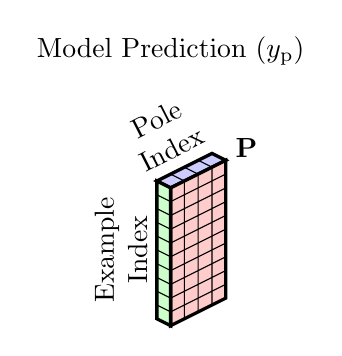
\begin{tikzpicture}[scale=0.175]
		\node at (0,7) {Model Prediction ($y_{\text{p}}$)};
        % Top
        \begin{scope}[
            yshift=-83,every node/.append style={
            yslant=0.5,xslant=-1},yslant=0.5,xslant=-1
            ]
            \filldraw[fill=blue!20] (0,0) rectangle (4, 1);
            \draw[step=1, black] (0,0) grid (4,1); %defining grids
            \draw[black,very thick] (0,0) rectangle (4,1);%marking borders
        \end{scope}
        \begin{scope}[
            yshift=-83,every node/.append style={
            yslant=0,xslant=0},yslant=0.5,xslant=0
            ]
            \filldraw[fill=red!20] (0,0) rectangle (4, -10);
            \draw[step=1, black] (0,0) grid (4,-10); %defining grids
            \draw[black,very thick] (0,0) rectangle (4,-10);%marking borders
        \end{scope}
        \begin{scope}[
            yshift=-83,every node/.append style={
            yslant=0,xslant=0},yslant=-0.5,xslant=0
            ]
            \filldraw[fill=green!20] (0,0) rectangle (-1, -10);
            \draw[step=1, black] (0,0) grid (-1,-10); %defining grids
            \draw[black,very thick] (0,0) rectangle (-1,-10);%marking borders
            \node[align=center,rotate=90,anchor=south] at (-1,-5) {Example\\ Index};
        \end{scope}
        
        \draw (-0.5,1.0) node[rotate=27,align=center] {Pole\\ Index};
        \node at (5.5,0) {$\mathbf{P}$};
        \end{tikzpicture}
        \hspace{0.25in}
        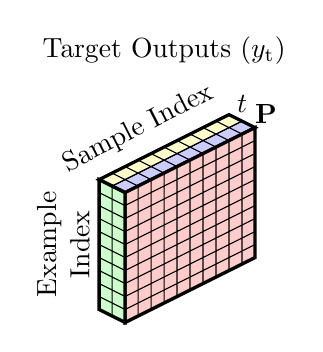
\begin{tikzpicture}[scale=0.165]
        \node at (3,8) {Target Outputs ($y_{\text{t}}$)};
        % Top
        \begin{scope}[
            yshift=-83,every node/.append style={
            yslant=0.5,xslant=-1},yslant=0.5,xslant=-1
            ]
            \filldraw[fill=blue!20] (0,0) rectangle (10, 1);
            \filldraw[fill=yellow!20] (0,1) rectangle (10, 2);
            \draw[step=1, black] (0,0) grid (10,2); %defining grids
            \draw[black,very thick] (0,0) rectangle (10,2);%marking borders
        \end{scope}
        \begin{scope}[
            yshift=-83,every node/.append style={
            yslant=0,xslant=0},yslant=0.5,xslant=0
            ]
            \filldraw[fill=red!20] (0,0) rectangle (10, -10);
            \draw[step=1, black] (0,0) grid (10,-10); %defining grids
            \draw[black,very thick] (0,0) rectangle (10,-10);%marking borders
            \node[xshift=4pt,yshift=5pt] at (10,0) {$\mathbf{P}$};
            \node[xshift=0pt,yshift=11pt] at (9,0) {$t$};
        \end{scope}
        \begin{scope}[
            yshift=-83,every node/.append style={
            yslant=0,xslant=0},yslant=-0.5,xslant=0
            ]
            \filldraw[fill=green!20] (0,0) rectangle (-2, -10);
            \draw[step=1, black] (0,0) grid (-2,-10); %defining grids
            \draw[black,very thick] (0,0) rectangle (-2,-10);%marking borders
            \node[align=center, rotate=90,anchor=south] at (-2,-5) {Example\\ Index};
        \end{scope}
        
        \draw (1,2) node[rotate=27] {Sample Index};
        \end{tikzpicture}
	}
	\caption{Model Prediction and Target Outputs}
	\label{fig:bl-in-out}
\end{figure}


Training the B\`ezier CNN is different from standard neural networks as the model predictions and the target outputs for training are differently shaped tensors as shown in Fig. \ref{fig:bl-in-out}. Where the image-to-point CNN was only responsible for the steering wheel angle $\theta_{\text{steering}} \in \mathbb{R}^1$, the image-to-curve CNN outputs poles $\mathbf{P}_k$ to form the B\`ezier curve hence the CNN output needs to exist in $\mathbb{R}^{(d+1)\times 1}$ space. To accomplish this, the last two layers are changed from the image-to-point CNN to the image-to-curve CNN with the polynomial output being a cubic with the resulting network architecture being shown in Table \ref{tab:i2c-arch}. For the target outputs during the training session, both the point and associated non-dimensional parameter $t$ value must be recorded. This leads leads to a mismatch in dimension size where, assuming the first tensor dimension is the example index, the second dimension of the tensors do not match. The model output has the second dimension reserved for indexing the poles forming the curve while the target output uses the second dimension to index the sample recorded points to fit the curve to.

Previous work rectified this dimensional discrepancy by generated output points $\mathbf{B}$ using a matrix representation $\mathbf{B} = \mathbf{A}(\mathbf{t},d) \mathbf{P}$ where $\mathbf{A}(\mathbf{t},d)$ is the matrix whose elements are $(1-t)^{d-k}t^k \genfrac(){0pt}{0}{d}{k}$ from \eqref{eq:bezier-curve} determining points by the matrix of output poles $\mathbf{P}$ and the corresponding parameter vector $\mathbf{t}$ \cite{trent2020iros}. While this implementation is simple, readily converted to a graph structure for GPU training, and easily integratable with preexisting loss functions it overly constrains the outputs as $\mathbf{A}$ needs to be determined a priori so the sampling can only happen at predetermined points. This work instead uses a custom implementation with functional mapping in Tensorflow 2.x to implement \eqref{eq:bl} which is sum of squared errors for arbitrary $n$ dimensional point spaces. As the implementation is a functional mapping, it is a more flexible approach that is robust to unique time window sampling spaces as well as ragged tensors i.e. the number of samples in a time window could potentially be different. A visual comparison of the model predicted tensors and the target outputs for applying \eqref{eq:bl} is shown in Fig. \ref{fig:bl-in-out} and the recorded steering wheel angle values have been been mapped to $[-1,\ 1]$ such that the extreme angles are $\pm 45^\circ$ degree turns so that the poles can allow for an intermediate point in the time window to achieve the vehicle limit of $\pm 30^\circ$ degree turns starting from a non-extreme value.

\begin{equation}
\label{eq:bl}
\begin{split}
\mathcal{L}_\mathbf{B}&(y_{\text{p}},\ y_{\text{t}}) = \sum_{e} \sum_{s} \left\| y_{\text{t}}(e,s,1:) -  \right. \\
&\left. \sum_{k=0}^d (1 - y_{\text{t}}(e,s,0))^{d-k} y_{\text{t}}(e,s,0)^k y_{\text{p}}(e,k,:) \right\|_2^2\\
\end{split}
\end{equation}

\subsection{Training}

The dataset is randomly split into a train set of 9 videos and a test set of 2 videos. Each of the videos have output keys generated in previous work where each video frame is matched to a recorded steering wheel angle. Since loading in all of the videos at once is resource expensive as the available hardware for this work only has roughly 2 Gigabytes of RAM available for the holding the input and output tensors, an unusual training scheme is performed. Rather than training over all frames of the 9 videos in batches as is traditional, the models are trained on a video as specified by sequentially iterating over an ordered list of videos before looping back and training on the list again. For training on a video, 200 frames are loaded into memory with a horizontal flip augmentation to yield 400 training examples for the model to train on. After training, the next 200 frames are loaded in training and this repeats until the model has trained on all 1,000 frames of a video. The specific training parameters and listings are shown in Table \ref{tab:training-parameters}.

\begin{table}[btp]
	\centering
	\caption{Training parameters}
	\begin{tabular}{|r|c|}
	\multicolumn{1}{c}{\textbf{Parameter}} & \multicolumn{1}{c}{\textbf{Value}} \\\hline
	Training Videos & [2, 9, 7, 8, 10, 1, 11, 6, 4] \\
	Loops over Training Set & 4\\
	Test Videos & 3 and 5 \\
	Epochs/200 Frames & 50 \\
	Batch Size & 256 \\
	Optimizer & ADAM \\
	Learning Rate & $\alpha=0.001$ \\
	Decay Rate & $\beta_1 = 0.9$, $\beta_2=0.999$ \\ \hline
	\end{tabular}
	\label{tab:training-parameters}
\end{table}

<<<Insert Training History>>>

\section{Experiments}

There are two methods to analyze the quality of the CNN; a quantitative accuracy check using the test videos and a qualitative check using a navigational track. These two methods are consistent with previous work \cite{bechtel2018} and allows for a fair comparison of the work.

\subsection{Model Accuracy}

Accuracy to the record values of the steering wheel is used to quantitatively evaluate the model quality for the various approaches. Accuracy is determined by iterating through all 2,000 total frames of the Video 3 and 5 of the test set in \cite{bechtel2018} and comparing continuous CNN outputs to their closest correspondence in the discrete $\lbrace -30^\circ,\ 0^\circ,\ 30^\circ\rbrace$ degree viable wheel angles with results shown in Tables \ref{tab:i2p-acc}, \ref{tab:i2bc-acc}, and \ref{tab:i2bp-acc}. The comparison previous work \cite{bechtel2018} using the same CNN architecture as the image-to-point network has shown accuracy of approximately 70\% although those models do not have normalization layer which is thought to be the reason why the baseline accuracy CNN are so poor in comparison. However, the results do show that using B\`ezier curves in the model networks do drastically improve the performance as they match the truth values at higher accuracy. Interestingly, reducing the ratio of control points to image frames down to a 1:1 drastically improved the CNN controller which indicates that using future steering angles greatly helps in improving the one-off prediction accuracy of image-to-point CNN controllers.


\begin{table}[btp]
	\centering
	\caption{Image-to-Point CNN Model (Acc: 20.45\%)}
	\begin{tabular}{|c|r|c|c|c|}
       \multicolumn{2}{c}{} & \multicolumn{3}{c}{\bfseries Model Predicted}\\\cline{3-5}
       \multicolumn{1}{c}{} & & \textbf{\textit{Left}} & \textbf{\textit{Center}} & \textbf{\textit{Right}}\\\hline
        \parbox[t]{2mm}{\multirow{3}{*}{\rotatebox[origin=c]{90}{\bfseries Record}}} & \textbf{\textit{Left}} & 48 & 31 & 21 \\\cline{3-5}
        & \textbf{\textit{Center}} & 156 & 156 & 188 \\\cline{3-5}
		& \textbf{\textit{Right}} & 54 & 136 & 205 \\\cline{3-5}\hline
	\end{tabular}
	\label{tab:i2p-acc}
\end{table}
    
\begin{table}[btp]
	\centering
	\caption{Image-to-Curve B\`ezier Model (Acc: 38.10\%) }
	\begin{tabular}{|c|r|c|c|c|}
		\multicolumn{2}{c}{} & \multicolumn{3}{c}{\bfseries Model Predicted}\\\cline{3-5}
		\multicolumn{1}{c}{} & & \textbf{\textit{Left}} & \textbf{\textit{Center}} & \textbf{\textit{Right}}\\\hline
		\parbox[t]{2mm}{\multirow{3}{*}{\rotatebox[origin=c]{90}{\bfseries Record}}} & \textbf{\textit{Left}} & 83 & 46 & 33 \\\cline{3-5}
		& \textbf{\textit{Center}} & 268 & 343 & 313 \\\cline{3-5}
		& \textbf{\textit{Right}} & 177 & 268 & 336 \\\cline{3-5}\hline
	\end{tabular}
	\label{tab:i2bc-acc}
\end{table}

\begin{table}[btp]
	\centering
	\caption{Image-to-Point B\`ezier Model (Acc: 66.75\%)}
	\begin{tabular}{|c|r|c|c|c|}
		\multicolumn{2}{c}{} & \multicolumn{3}{c}{\bfseries Model Predicted}\\\cline{3-5}
		\multicolumn{1}{c}{} & & \textbf{\textit{Left}} & \textbf{\textit{Center}} & \textbf{\textit{Right}}\\\hline
		\parbox[t]{2mm}{\multirow{3}{*}{\rotatebox[origin=c]{90}{\bfseries Record}}} & \textbf{\textit{Left}} & 60 & 111 & 9 \\\cline{3-5}
		& \textbf{\textit{Center}} & 48 & 667 & 261 \\\cline{3-5}
		& \textbf{\textit{Right}} & 13 & 223 & 608 \\\cline{3-5}\hline
	\end{tabular}
	\label{tab:i2bp-acc}
\end{table}

<<<Video of Results>>>

\subsection{Physical Driving}

Unfortunately the models could never be implemented on the platform in and with the previous software of \cite{bechtel2018}. There seems to be numerous packaging issues surrounding Tensorflow on the Raspberry Pi. The previous work used Python 2 but their installation instructions with for the wiringpi module are outdated as it installs into the now default Python 3. Python 3 cannot be used as Python 3.5 is now depreciated as of September of 2020 and Python 3.5 was the last version to work with Tensorflow 1.x but it is possible to install the wiringpi module for Python 2. This work was able to install Tensorflow 1.11.0 as a regular user, the wiringpi library as required by the radio-control car motor module needs to be run as the super user. Unfortunately, installation of Tensorflow 1.11.0 was not achievable as the super user as all attempts for installation hung on the grpcio module installation which has a known long, and apparently indefinite installation time.

\section{Results and Conclusions}

This work illustrated that the B\`ezier CNNs with either direct or indirect controllers will yield smoother results over classical CNN direct controllers. Regrettably, this still is only theoretical as the performance benefit has not been demonstrated on a physical platform.

\section{Future Work}

The DeepPicar-v2 dataset is initially limiting; wheel angles are only three variations and there is a one-to-one correspondence between wheel angles and video frames. Curve fitting to noisy data best works with more sampling of points. Rather than constructing the dataset by forming corresponding pairs, have two threads of data collection. The first thread is for the camera at a nominal operational rate for image-to-point usage and the second thread is for measure the wheel steering angle. Alternatively the original \cite{bechtel2018} could be modified by estimating intermediate point values to upsample the presented data from 20 Hz to a more effect sensor rate. Lastly, the B\`ezier CNNs still need to be tested on physical platform so it may require rewrites of the neural network portion of the controllers scripts in the original DeepPicar.

\bibliographystyle{IEEEtran}
\bibliography{final-report}

\end{document}
